\documentclass{standalone}
\usepackage{picture,color}
\usepackage{graphicx}
\graphicspath{{./EM_features/}}
\setlength{\unitlength}{1in}
\renewcommand{\rmdefault}{phv} % Arial
\renewcommand{\sfdefault}{phv} % Arial


\begin{document}
\begin{picture}(4.54, 5.18)(0,-5.28)

\put(0., -2.18){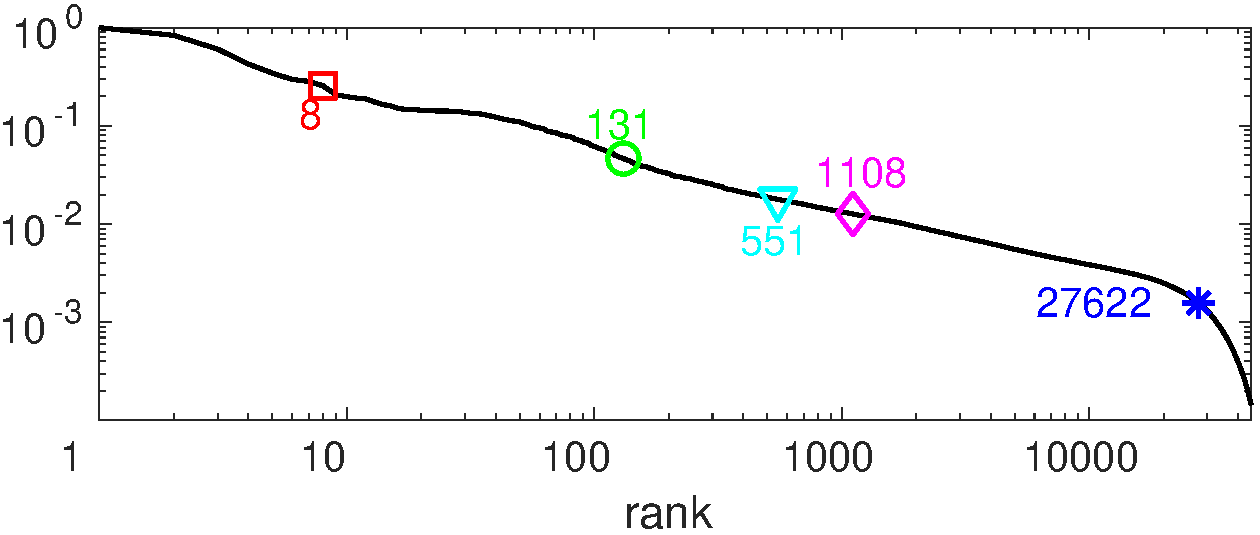
\includegraphics[height=1.93in]{nvoxels.pdf}}
\put(0.01, -0.28){\large\textbf{A}}
% \put(1.9, -0.25){$l1$ norm of EM footprints}
\put(1.3, -0.25){Relative size of EM components}

% slice number 
\put(0.9, -2.3){{slice 1}}
\put(2.3, -2.3){{slice 2}}
\put(3.7, -2.3){{slice 3}}
\put(0.01, -2.3){\large\textbf{B}}

% neuron 1
\put(0.35, -2.92){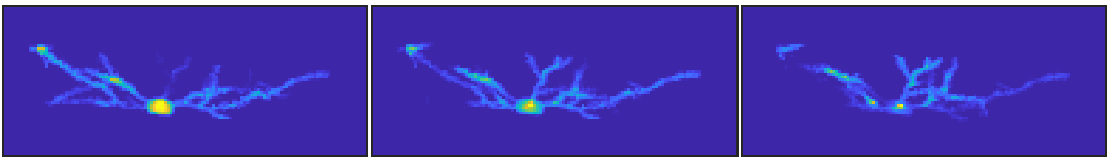
\includegraphics[width=4.2in]{example_1.pdf}}
\put(0.2, -2.64){\rotatebox{90}{\color{red}8}}

% neuron 2 
\put(0.35, -3.51){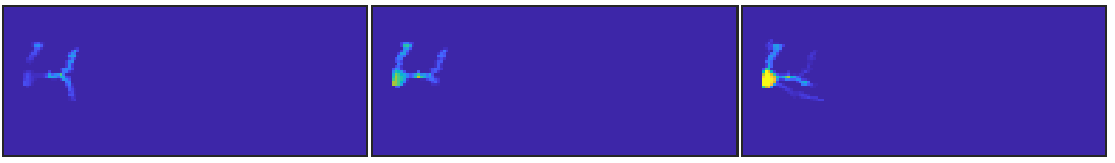
\includegraphics[width=4.2in]{example_2.pdf}}
\put(0.2, -3.31){\rotatebox{90}{\color{green}131}}

% neuron 3 
\put(0.35, -4.10){
\includegraphics[width=4.2in]{example_3.pdf}}
\put(0.2, -3.92){\rotatebox{90}{\color{cyan}551}}

% neuron 4
\put(0.35, -4.69){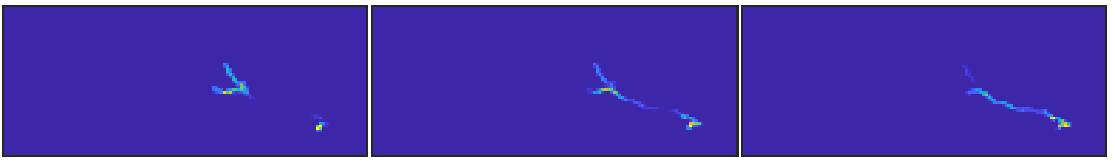
\includegraphics[width=4.2in]{example_4.pdf}}
\put(0.2, -4.57){\rotatebox{90}{\color{magenta}1108}}

% neuron 5
\put(0.35, -5.28){
\includegraphics[width=4.2in]{example_5.pdf}}
\put(0.2, -5.23){\rotatebox{90}{\color{blue}27622}}
\end{picture}
\end{document}\grid
